\documentclass{report}
\usepackage[T1]{fontenc} 
\usepackage[utf8]{inputenc} 
\usepackage{lmodern}
\usepackage [frenchb]{babel}
% Pour pouvoir utiliser 
\usepackage{ucs}
%claude.jard@univ-nantes.fr
%23h59 9 novembre
\usepackage{tikz}
\usepackage{epsfig}
\usepackage{amsbsy,amsmath}
\usepackage{rotating}
\usepackage{graphicx}
\usepackage{color}
\usepackage{amsbsy}
\usepackage{natbib}
\usepackage{tikz}
\usepackage{textcomp}
\usepackage{graphicx}
\usepackage{keystroke}
\usepackage{amssymb}
\usepackage{amsmath}
%\renewcommand{\thesection}{\arabic{section}} % numérotation des sections	
\usepackage[cc]{titlepic} %rajouter le logo dans la page de garde
\usepackage{url} % Pour avoir de belles url
\usepackage[a4paper]{geometry}
\usepackage[linktocpage]{hyperref}
% Pour pouvoir faire plusieurs colonnes
\usepackage {multicol}
%Pour faire plusieurs lignes
\usepackage{multirow}
\usepackage{slashbox}
% Pour mettre du code source
\usepackage {listings}
% Pour pouvoir passer en paysage
\usepackage{lscape}	

% Pour pouvoir faire plusieurs colonnes
\usepackage {multicol}

% POur crééer un index
\usepackage{makeidx}

%Pour taper des algorithme en pseudo code
%\usepackage{algorithm,algorithmic}

%insertion de pdf
\usepackage{pdfpages}

%Utilisation d'acronyme
\usepackage{acronym}

\usepackage{fancyhdr}
\pagestyle{fancy}
\usepackage{lastpage} %numérotation type k/n
\setlength{\topmargin}{0,1cm}
\setlength{\headsep}{1,8cm}
%\addtolength{\textheight}{cm}
\renewcommand{\footrulewidth}{0.5pt} % trait horizontal
%\renewcommand{\headrulewidth}{1pt} % suppresion du trait horizontal dans l'entête
\lfoot{Projet Formal Software}
\cfoot{\thepage \hspace{0.15cm}sur  \pageref{LastPage} } % numérotation des pages
\rfoot{A.\textsc{Marguerite} \& R.\textsc{Rincé}}
\fancyhead[L]{\hspace{-0.3cm}
\includegraphics[scale=0.15]{img/logouniv.eps}} %logo entête !


\fancypagestyle{plain}{% 1ères pages des chapitres:
  % \fancyhead{} % supprime l’entete...
  % \renewcommand{\headrulewidth}{0pt} % ...et le filet
}




\hypersetup{
  backref=true,
  %permet d'ajouter des liens dans...
  pagebackref=true,%...les bibliographies
  hyperindex=true, %ajoute des liens dans les index.
  colorlinks=true, %colorise les liens
  breaklinks=true, %permet le retour à la ligne dans les liens trop longs
  urlcolor= blue, %couleur des hyperliens
  citecolor=	cyan,
  bookmarks=true, %créé des signets pour Acrobat
  bookmarksopen=true,
  %si les signets Acrobat sont créés,
  %les afficher complètement.
  pdftitle={FormalSoftware}, %informations apparaissant dans
  pdfauthor={MARGUERITE Alain\\ RINCE Romain},
  %dans les informations du document
  pdfsubject={Doc}
  %sous Acrobat.
}

\makeindex
%%%% debut macro pour enlever le nom chapitre %%%%
\makeatletter
\def\@makechapterhead#1{%
  \vspace*{50\p@}%
          {\parindent \z@ \raggedright \normalfont
            \interlinepenalty\@M
            \ifnum \c@secnumdepth >\m@ne
            \Huge\bfseries \thechapter\quad
            \fi
            \Huge \bfseries #1\par\nobreak
            \vskip 40\p@
}}

\def\@makeschapterhead#1{%
  \vspace*{50\p@}%
          {\parindent \z@ \raggedright
            \normalfont
            \interlinepenalty\@M
            \Huge \bfseries  #1\par\nobreak
            \vskip 40\p@
}}
\makeatother
%%%% fin macro %%%%
%Couverture 
\widowpenalty=10000
\clubpenalty=10000
\hyphenation{permet-tant}

\title{ {\huge \textsc{Formal Software}} \\Master ALMA 2\up{eme} année \\\vspace{3cm} \emph{Projet : Réalisation d'une application à automates} \\ {\small Encadrant : C.\textsc{Jard}}\vspace{3cm}}
\titlepic{ 
\includegraphics[scale=0.2]{img/logouniv}}
\author{A.\textsc{Marguerite}\\ R.\textsc{Rincé}\vspace{3cm}}
\date{Université de Nantes \\ 2 rue de la Houssinière, BP92208, F-44322 Nantes cedex 03, FRANCE}
%\vspace{20cm}


\newcommand{\cf}{\emph{cf}.}


\begin{document}
\maketitle
\renewcommand{\labelitemi}{$\bullet$} 

\clearpage

\tableofcontents
\clearpage

%\chapter*{Remerciements}
\phantomsection
\addcontentsline{toc}{section}{Remerciements}
 TODO TODO TODO TODO TODO TODO TODO TODO TODO TODO TODO TODO TODO TODO TODO TODO TODO TODO TODO TODO TODO TODO

 TODO TODO TODO TODO TODO TODO TODO TODO TODO TODO TODO TODO TODO TODO TODO TODO TODO TODO TODO TODO

\chapter{Introduction}\label{chap:Intro}

\section{Problématiques}
Les problèmes d'inter-opérabilité et de réutilisabilité font partie des problématiques majeures des systèmes informatiques. La programmation objet ne parvient pas à répondre à ces problématiques à cause notamment de ses propriétés de granularité et de fort couplage. Les problèmes de cohésions (pas d'explications des besoins requis) sont un frein à l'utilisation de la programmation objet à grande échelle. 

Parmi les solutions à ces problématiques les architectures à composants sont des alternatives efficaces. Un composant, entité principale, correspond par définition à une ou plusieurs fonctionnalités. Il est donc possible de le concevoir et de le pré-tester de manière indépendante. La coopération entres composant est alors plus aisée. De plus un composant possède un couplage lâche. Cette propriété garantissant l'inter-opératibilté est permise par l'utilisation d'interfaces entre composants. 

\section{Présentation du sujet}
Le module \textsc{Architectures and Components} nous propose une étude de la programmation par composants. L'objectif de ce Projet/TP  est de réaliser un Home Architecture Description Language, et d'implémenter une architecture classique \emph{Clients-Serveur}. La démarche proposée pour atteindre cet objectif est composée de trois étape : 


\begin{enumerate}
\item 
Réalisation du M2 :\hfill \\
Il s'agit d'un méta-modèle de l'architecture en composants.  
\item
Réalisation du M1 :\hfill \\
À partir du méta-modèle précédement réalisé, nous pouvons proposer une instance de ce dernier et obtenir un modèle. Nous choisirons ici de modéliser une application classique \emph{Client-Serveurs}.  
\item
Réalisation du M0 :\hfill \\
Dernière étape, elle consiste à l'implémentation du M1 et de coder concrétement qui y sont modélisées.
\end{enumerate}

Dans ce rapport nous détaillerons chaque étape la modélisation proposée puis l'implémentation.

\chapter{Implémentation du protocole}

\section{Solutions choisies}
Le langage choisi est \textsc{JAVA}. Les motivations de ce choix sont les suivantes : la facilité  ainsi que la mise à disposition par \textsc{JAVA} de moniteurs. Effet, la classe \texttt{UnicastRemoteObject} propose les objets \textit{RMI} (Remote Method Invocation). Il s'agit d'objets \og distants \fg{} auxquels des appels de méthodes peuvent être effectués comme si l'objet était local. De plus  l'implémentation des objets \texttt{RMI}  utilise les moniteurs. Ce mécanisme, garantissant l'emploi de canaux de type \texttt{FIFO}, est donc approprié pour le protocole de ce projet.  

\section{Implémentation}

\subsection{Partie serveur}
La partie \og serveur \fg{} est implémentée par la classe \texttt{IA}, la figure \ref{fig:ia} illustre que cette classe hérite de l'interface \texttt{IIA}. Cet héritage est indispensable pour l'utilisation d'objet \texttt{RMI}. Les signatures des méthodes que l'interface contient sont les moyens pour le client de dialoguer avec le serveur. Bien sûr le client doit avoir la connaissance de cette interface.

 \begin{figure}[htb]
   \centering
   
\includegraphics[scale=.5]{img/ia.eps}
   \caption{Partie serveur}
   \label{fig:ia}
 \end{figure}
\clearpage
\paragraph{L'IHM serveur} (\cf{} figure \ref{fig:ihmIA}) est composée de deux parties : 
\begin{enumerate}
\item 
Partie supérieure : Affichage de l'automate serveur.
\item
Partie inférieure : Affichage textuel des événements.
\end{enumerate}
L'utilisateur n'a en théorie aucune interaction possible avec le serveur. Dans un soucis pratique nous avons cependant rajouté un bouton \texttt{QUIT} permettant de quitter et réinitialiser le serveur.
 \begin{figure}[htb]
   \centering
   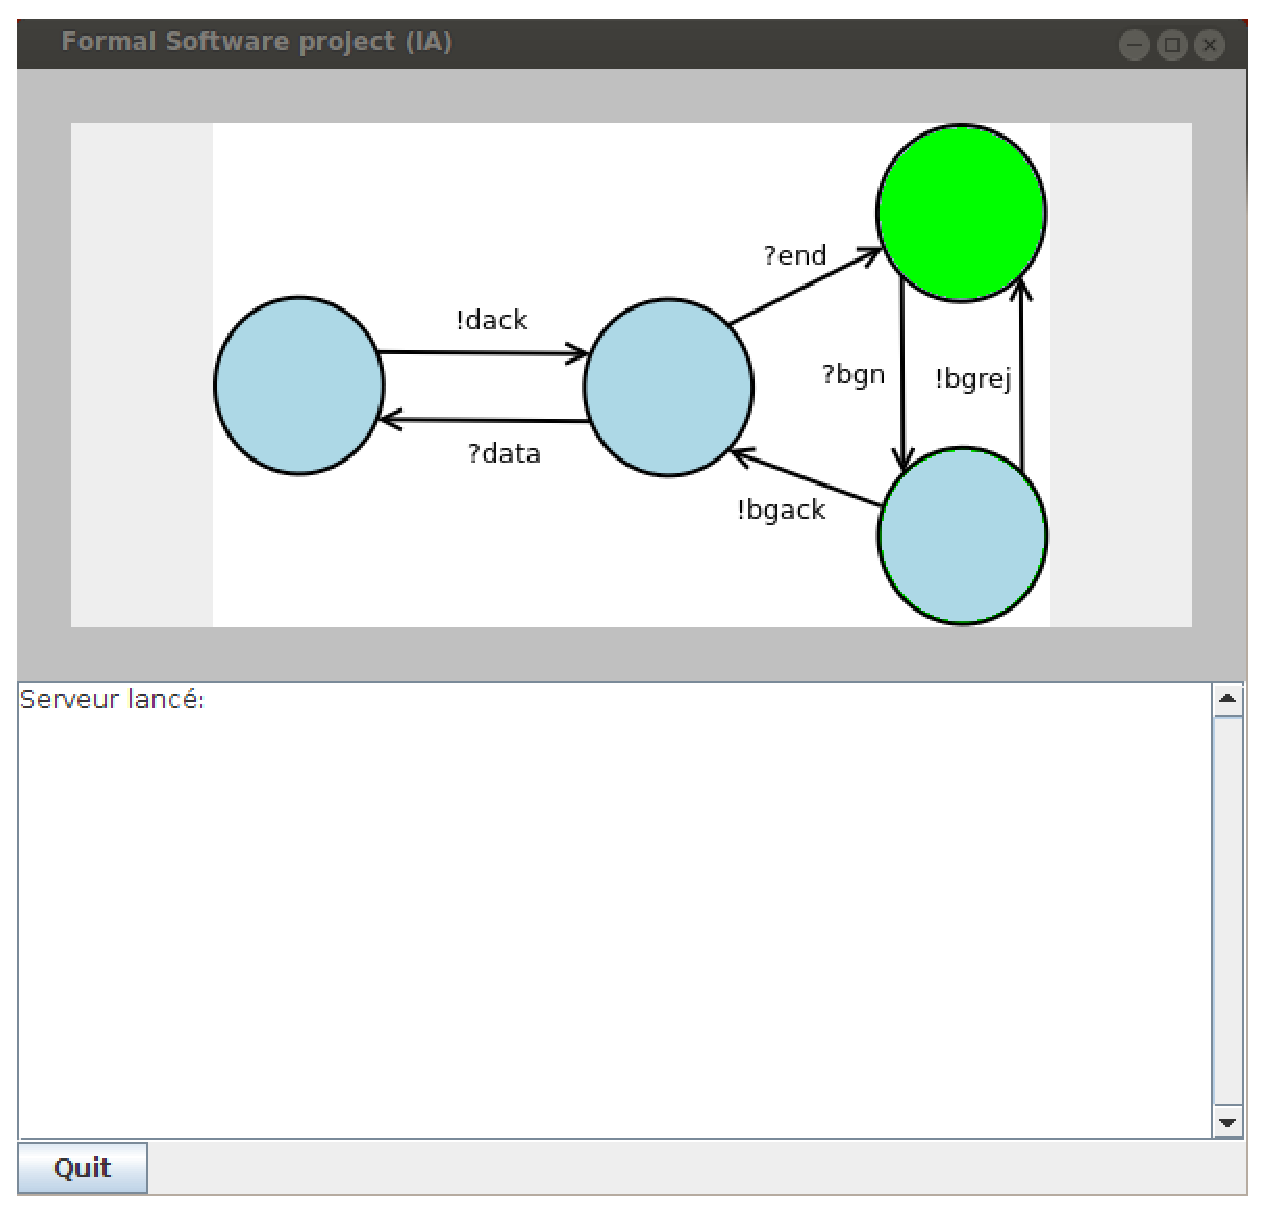
\includegraphics[scale=.5]{img/ihmIA.eps}
   \caption{IHM du serveur}
   \label{fig:ihmIA}
 \end{figure}


\clearpage
\subsection{Partie client}
\paragraph{L'IHM client}(\cf{} figure \ref{fig:ihmCLIENT}) est composée de trois parties : 
\begin{enumerate}
\item 
Partie supérieure : Affichage de l'automate client.
\item
Partie centrale : Affichage textuel des événements.
\item 
Partie inférieure : Boutons de contrôle.
\end{enumerate}

 \begin{figure}[htb]
   \centering
   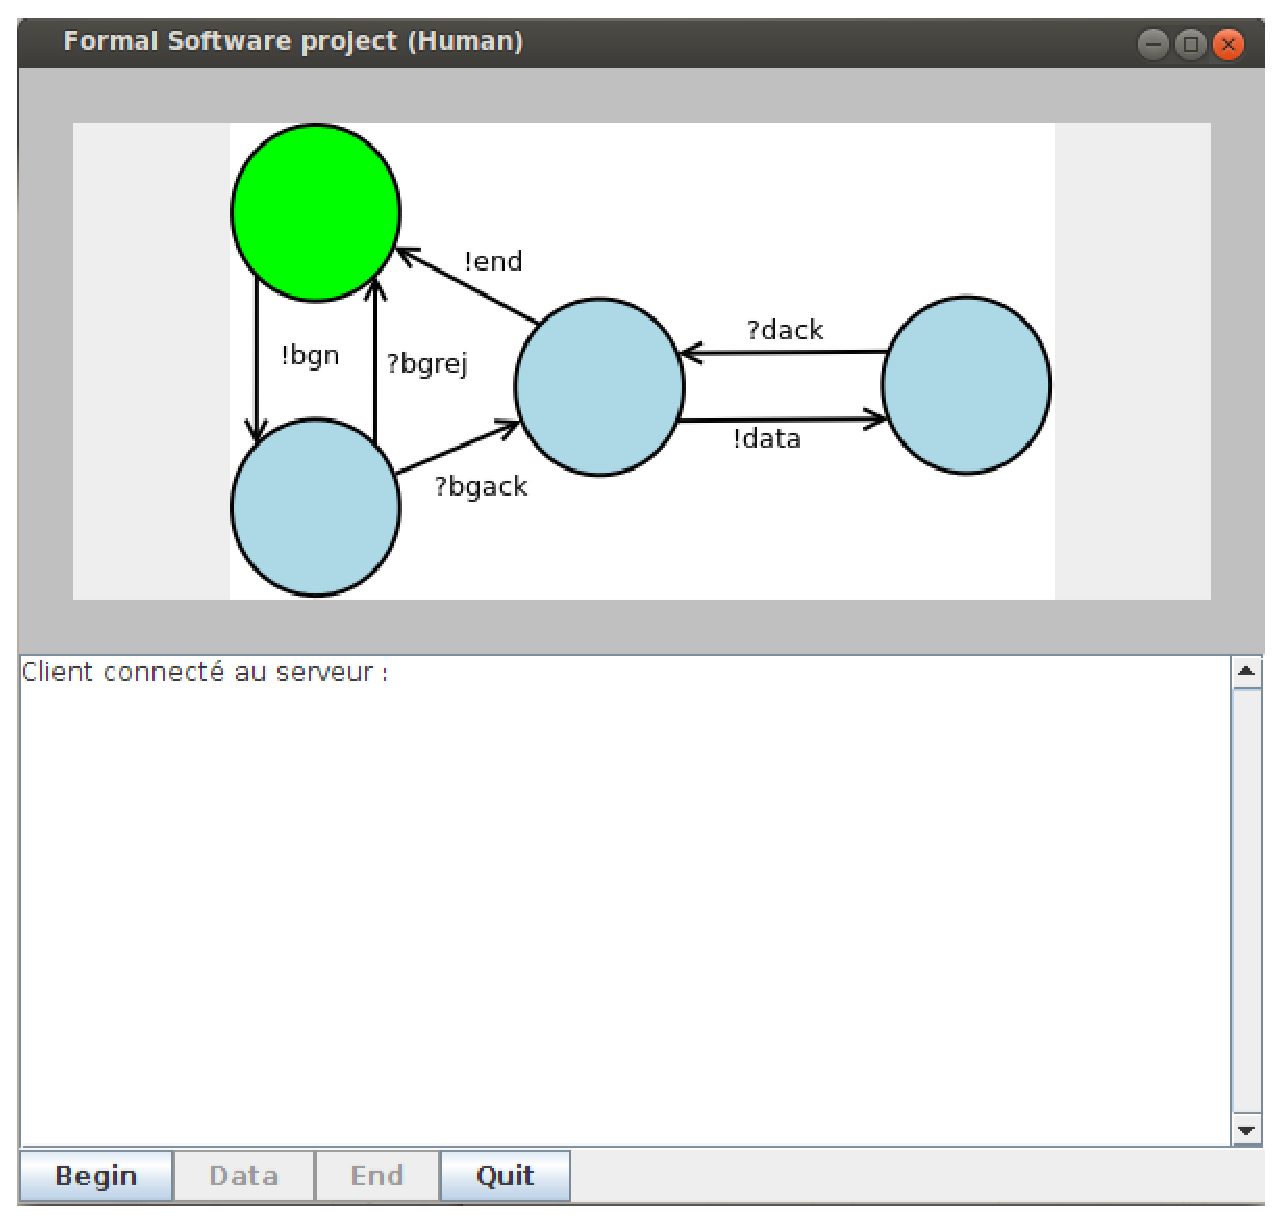
\includegraphics[scale=.5]{img/ihmCLIENT.eps}
   \caption{IHM du client}
   \label{fig:ihmCLIENT}
 \end{figure}
Les boutons de contrôles :  \texttt{BEGIN}, \texttt{DATA} et \texttt{END} correspondent respectivement aux opérations : \texttt{sendBegin()}, \texttt{sendData()} et \texttt{sendEnd()}, définies dans l'interface \texttt{IIA} (\cf{} figure \ref{fig:ia}). L'utilisateur peut par ses boutons \og tirer \fg{} les transitions de l'automate.

\section{Problèmes rencontrés}
\subsection{Mutli-threading}
Au cours du développement de l'application, il était nécessaire d'effectuer systématiquement des tests pour vérifier si les automates étaient dans un état cohérent. Dans un souci pratique nous avons effectué ces tests en local. L'objet \og distant \fg{} \texttt{RMI} était donc lié au \texttt{localhost} (\verb+127.0.0.0+). Ainsi les messages entre le client et le serveur mettaient en moyenne moins d'un millième de seconde pour rejoindre leur destinataire (modulo la précision de l'API de mesure temporelle de \textsc{JAVA}).

Un des premiers problèmes que nous avons rencontré dans le développement l'application était donc celui de \og ralentir \fg{} ces opérations afin de vérifier la cohérence des automates.

De plus les rafraîchissements des espaces de visualisation des différents automates posèrent eux aussi de nombreux problèmes. La couche \texttt{SWING} de \textsc{JAVA} en charge de l'implémentation des interfaces graphiques, est elle-même un thread à part entière. Une des difficultés était donc de synchroniser au sein d'un même thread application, le thread \og vue \fg{} (la couche \texttt{SWING}) avec la couche \og métier \fg{} (algorithmes des automates et de leurs communications).


% LocalWords:  Implémentation UnicastRemoteObject RMI Remote Method
% LocalWords:  l'implémentation FIFO IA IIA L'IHM QUIT IHM BEGIN END
% LocalWords:  sendBegin sendData sendEnd Mutli-threading localhost
% LocalWords:  modulo l'API thread tread

%\chapter{Implémentation du M1}
Dans ce chapitre nous définirons une application \textit{Client-Serveur} en implémentant le méta-model proposé au chapitre \ref{chap:M2}.

\section{Démarche modélisation M1}
L'énoncé du projet/TP nous propose un serveur avec les fonctionnalités suivantes :

\begin{itemize}
\item \verb+ConnexionManager+ :   Gestion des connexions. 
\item  \verb+Database+ :  Gestion de la base de données.
\item \verb+SecurityManager+ :  Gestion d'un système de sécurité.
\end{itemize}

Un composant étant par définition la spécification d'une fonctionnalités, chacune des fonctionnalités précedement listées est un \verb+Composant+. Chaque service de chaque composant a son port requis relié au rôle fournis  du connecteur ( et inversement pour les ports fournis et rôles requis).

Les liaisons est ces différents composant et le client sont explicitées dans la figure \ref{fig:desSer}.
\begin{figure}[htb]
  \centering
  \includegraphics[scale=0.32]{img/DescribServeur}
  \caption{Description du Serveur}
  \label{fig:desSer}.
\end{figure}


\subsection{ConnexionManager}
Ce composant possède les services suivants : 
\begin{itemize}
\item 
  \verb+ServiceFExternalSocket+ : Fournit une connexion au serveur.
\item 
  \verb+ServicerDDBQuery+ :  requière une réponse de la base de données (requête SQL).
\item 
  \verb+ServiceRSecurityManager+ :  requière une validation de l'authentification
\end{itemize}


\subsection{Database}
Ce composant possède les services suivants : 
\begin{itemize}
\item 
  \verb+ServiceFSecurityManagement+ :  fournit une réponse à la requête de sécurité.
\item 
  \verb+ServicerFExecuteSQL+ :  fournit une réponse à une requête du client (par le ConnexionManager).
\end{itemize}

\subsection{SecurityManager}
Ce composant possède les services suivants : 
\begin{itemize}
\item 
  \verb+ServiceFSecurityAuth+ : fournit une validation de la demande de connexion.
\item 
  \verb+ServicerSecurityManager+ :  requière une réponde de sécurité de la base de données (requête SQL).
\end{itemize}

\section{Diagramme M1}
\pagestyle{empty}
%\newgeometry{a3paper}
\begin{figure}[htb]
  \centering
  \includegraphics[scale=0.20]{img/M1}
  \caption{Model (M1)}
  \label{fig:M1}
\end{figure}

\chapter{Conclusion}\label{chap:COnc}
À ce stade, la modélisation de notre méta-modèle (\cf{} chapitre \ref{chap:M2}) nous a permis de générer un modèle pour notre application \textit{Clients-Serveur} (\cf{} chapitre \ref{chap:M1}). Par la suite il sera nécessaire de passer à l'étape 3 présentée au chapitre \ref{chap:Intro}. C'est à dire  d'implémenter le méta-modèle M2 en JAVA.

La création de l'application \textit{Clients-Serveur} repose sur l'héritage des classes du méta-modèle. Enfin l'instanciation concrète de ses classes achèvera l'implémentation de notre application.

% LocalWords:  méta-modèle Clients-Serveur l'instanciation
% LocalWords:  l'implémentation



\listoffigures
% Pour finir l'interligne de 1,5
%\bibliographystyle{alpha}
%\bibliography{biblio.bib}


\end{document}
